\documentclass[10pt]{article}
\usepackage{parskip}
\usepackage[utf8]{inputenc}
\usepackage[left=2.00cm, right=2.00cm, top=2.00cm, bottom=2.00cm]{geometry}
\usepackage[spanish]{babel}
\usepackage{graphicx,subfig}
\usepackage{fancyhdr}
\usepackage{pgfplots}
\usepackage[rightcaption]{sidecap}
\usepackage[font=small,labelfont=bf]{caption}
\graphicspath{{Imagenes/}}
\usepackage{enumerate} 
\usepackage{multicol}
\usepackage{tabularx}
\usepackage{amssymb}
\usepackage{adjustbox}
\usepackage{amsmath}
\usepackage{cancel}
\begin{document}


\pagestyle{fancy}
\cfoot{}


%Cabeceras
\rhead{Oscilador Armónico.}
\lhead{}

%Portada
\begin{titlepage}
	\newgeometry{
		left=25mm,
		right=25mm,
		top=5mm,
		bottom=30mm,
		headheight = 0 mm
	}

	\begin{figure}[t]
		\subfloat{
\includegraphics[width=0.15\textwidth]{Logo_IPN}}
		\hspace{0.6\textwidth}
		\subfloat{
\includegraphics[width=0.22\textwidth]{LogoEsime}}
	\end{figure}

	\centering
	{\bfseries\Huge Instituto Politécnico Nacional. \par}
	\vspace{1cm}
	{\scshape\Large Ingeniería en Comunicaciones y Electrónica. \par}
	\vspace{0.3cm}
	{\scshape\Large Laboratorio de Ondas Mecanicas.  \par}
	\vspace{1cm}
	{\scshape\Huge Señor Doctor Slinky \par}
	\vspace{1cm}
	{\itshape\Large Oscilador Armonico. \par}
	{\Large 2CM13\par}
	\vfill
	{\Large Autores: \par}
	{\Large Hernández Huerta Jose Emilio. \par}
	{\Large Hernández Sanluis Danna Estefany.  \par}
	{\Large Garduño Bejarano Nataly. \par}
	{\Large Mojica Reyes Rogelio.\par}
	{\Large Morlan Juárez Bruno Tonatiuh.  \par}
	{\Large Santos Marañón María Renée.\par}
	\vfill
	{\Large Sep 2023. \par}

\end{titlepage}

\tableofcontents
\newpage

\section{Resumen.}
Se realizaron una serie de experimentos relacionados con el movimiento armónico simple y el comportamiento de un resorte. Los experimentos se llevaron a cabo utilizando un resorte helicoidal y una serie de masas de diferente magnitud.  

\begin{multicols}{2}

\section{Objetivo.}
El objetivo general de esta práctica de laboratorio es estudiar y comprender el comportamiento de un sistema masa-resorte en movimiento armónico simple, así como determinar la constante de restitución del resorte y obtener la aceleración de la gravedad de la localidad mediante experimentos controlados y análisis de datos.
\section{Introducción.}

El conocimiento adquirido en esta práctica resulta relevante no solo desde una perspectiva académica, sino también en numerosos campos de la física y la ingeniería, donde el movimiento armónico simple es un concepto fundamental. Además, esta práctica ofrece la oportunidad de aplicar técnicas experimentales y de análisis de datos, fortaleciendo así las habilidades de los estudiantes en el ámbito de la investigación científica.


\section{Marco teórico.}
El Movimiento Armónico Simple (MAS) es un concepto fundamental en la física que describe el movimiento periódico y oscilatorio de un objeto alrededor de una posición de equilibrio. Este tipo de movimiento se encuentra en una amplia variedad de sistemas físicos y es esencial para comprender fenómenos como las vibraciones, las ondas, el movimiento de un péndulo y muchas otras aplicaciones en la ciencia y la ingeniería.(Fernández, s. f.)

Aquí hay algunas características clave del Movimiento Armónico Simple:

Oscilación Periódica: En el MAS, el objeto se mueve de un lado a otro en torno a una posición de equilibrio en un patrón repetitivo y predecible. Esto significa que el objeto vuelve una y otra vez a la misma posición en intervalos regulares de tiempo.(Simple Harmonic motion, s. f.

Fuerza Restauradora: El MAS ocurre cuando una fuerza restauradora proporcional a la distancia desde la posición de equilibrio actúa sobre el objeto. La dirección de esta fuerza es opuesta al desplazamiento del objeto desde la posición de equilibrio. En otras palabras, cuanto más se aleje el objeto de la posición de equilibrio, mayor será la fuerza que lo empuja de regreso hacia ella.(Simple Harmonic motion, s. f.)

Movimiento Armónico Simple Lineal: En el MAS, la relación entre la fuerza restauradora y la posición del objeto es lineal. Esto se rige por la ley de Hooke, que establece que la fuerza ejercida por un resorte es directamente proporcional a la elongación o compresión del resorte.(Simple Harmonic motion, s. f.

Amplitud: La amplitud es la máxima distancia que el objeto se desplaza desde la posición de equilibrio en cada ciclo de oscilación. Es un parámetro importante que determina la magnitud del movimiento.

Periodo y Frecuencia: El periodo (T) es el tiempo que tarda el objeto en completar un ciclo completo de oscilación, es decir, volver a la misma posición y velocidad. La frecuencia (f) es el número de ciclos completos por unidad de tiempo y se relaciona inversamente con el periodo mediante la ecuación f = 1/T.(Simple Harmonic motion, s. f.)

Desfase: El desfase es la diferencia en la fase de dos movimientos armónicos simples. Puede describir cómo dos oscilaciones se sincronizan o se desplazan una con respecto a la otra. (Simple Harmonic motion, s. f.)
\subsection{ Movimiento Armónico Simple}
\begin{center}
	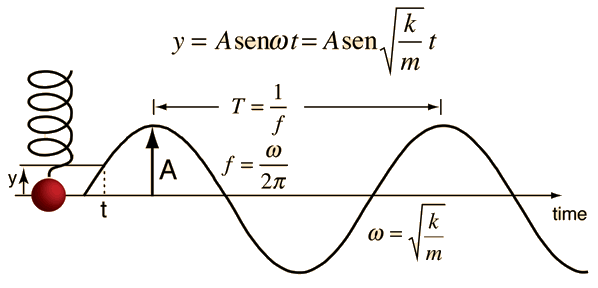
\includegraphics[width=8cm, height=5cm]{Imagenes/mas.png}
	\captionof{figure}{Movimiento Armónico Simple.}
\end{center}



\section{Experimento 1. Determinación de la constante de restitución del resorte $(k)$}
Durante esta práctica se armo el dispositivo con el que íbamos a trabajar para poder hacer las determinaciones constantes de la restitución.
Para esto colocamos el resorte en la balanza de Jolly y tomamos un punto de referencia en la parte inferior del resorte ,el cual también nos apoyamos con un pequeño espejo que está en la balanza. 
\begin{center}
	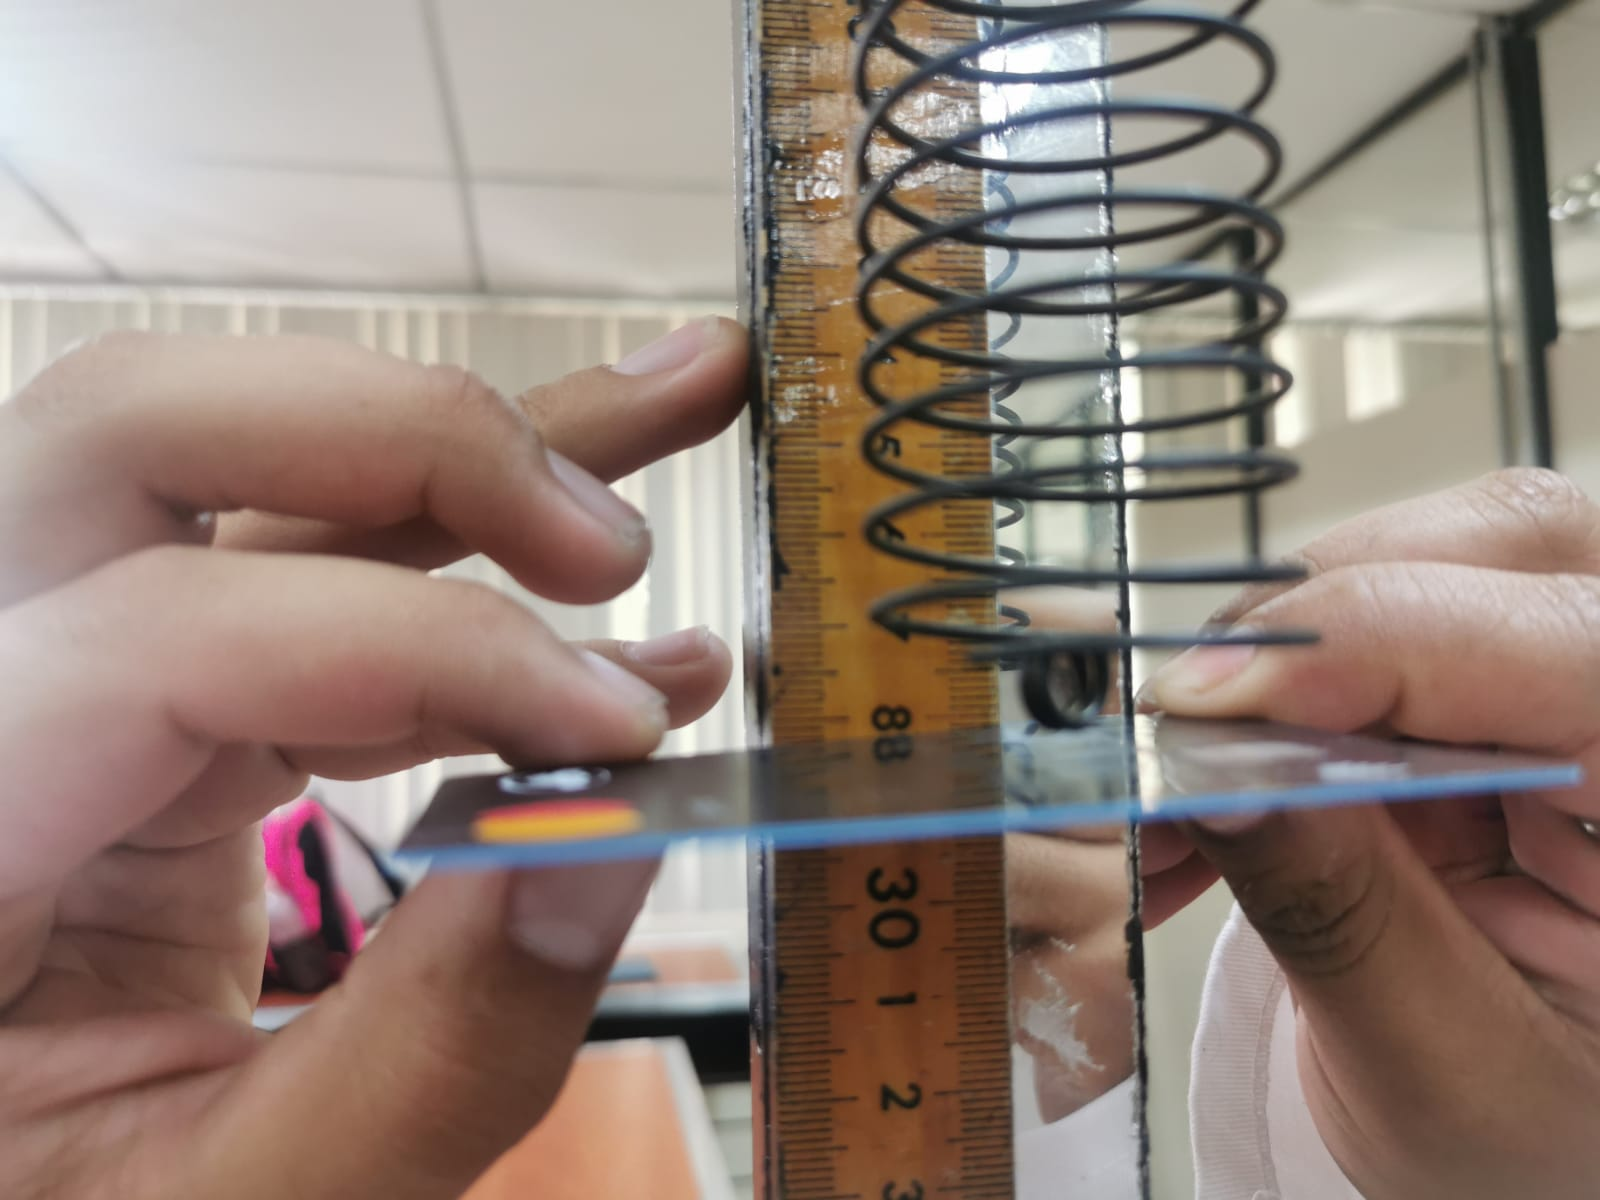
\includegraphics[width=4cm, height=7cm]{Imagenes/medida.jpeg}
	\captionof{figure}{Longitud inicial del resorte.}
\end{center}
Como segundo paso , colocamos una pesa de 50 g (0.050 kg) en la pequeña argolla que se encontraba al final del resorte y medimos la deformación($X_{1}$) que sufrió el resorte ,  este cálculo es la distancia que existe entre el punto  de referencia inicial y la nueva posición de el mismo punto .
El paso anterior lo repetimos varias veces con los pesos que nos marcaba la tabla que esta a continuación :
\begin{center}
	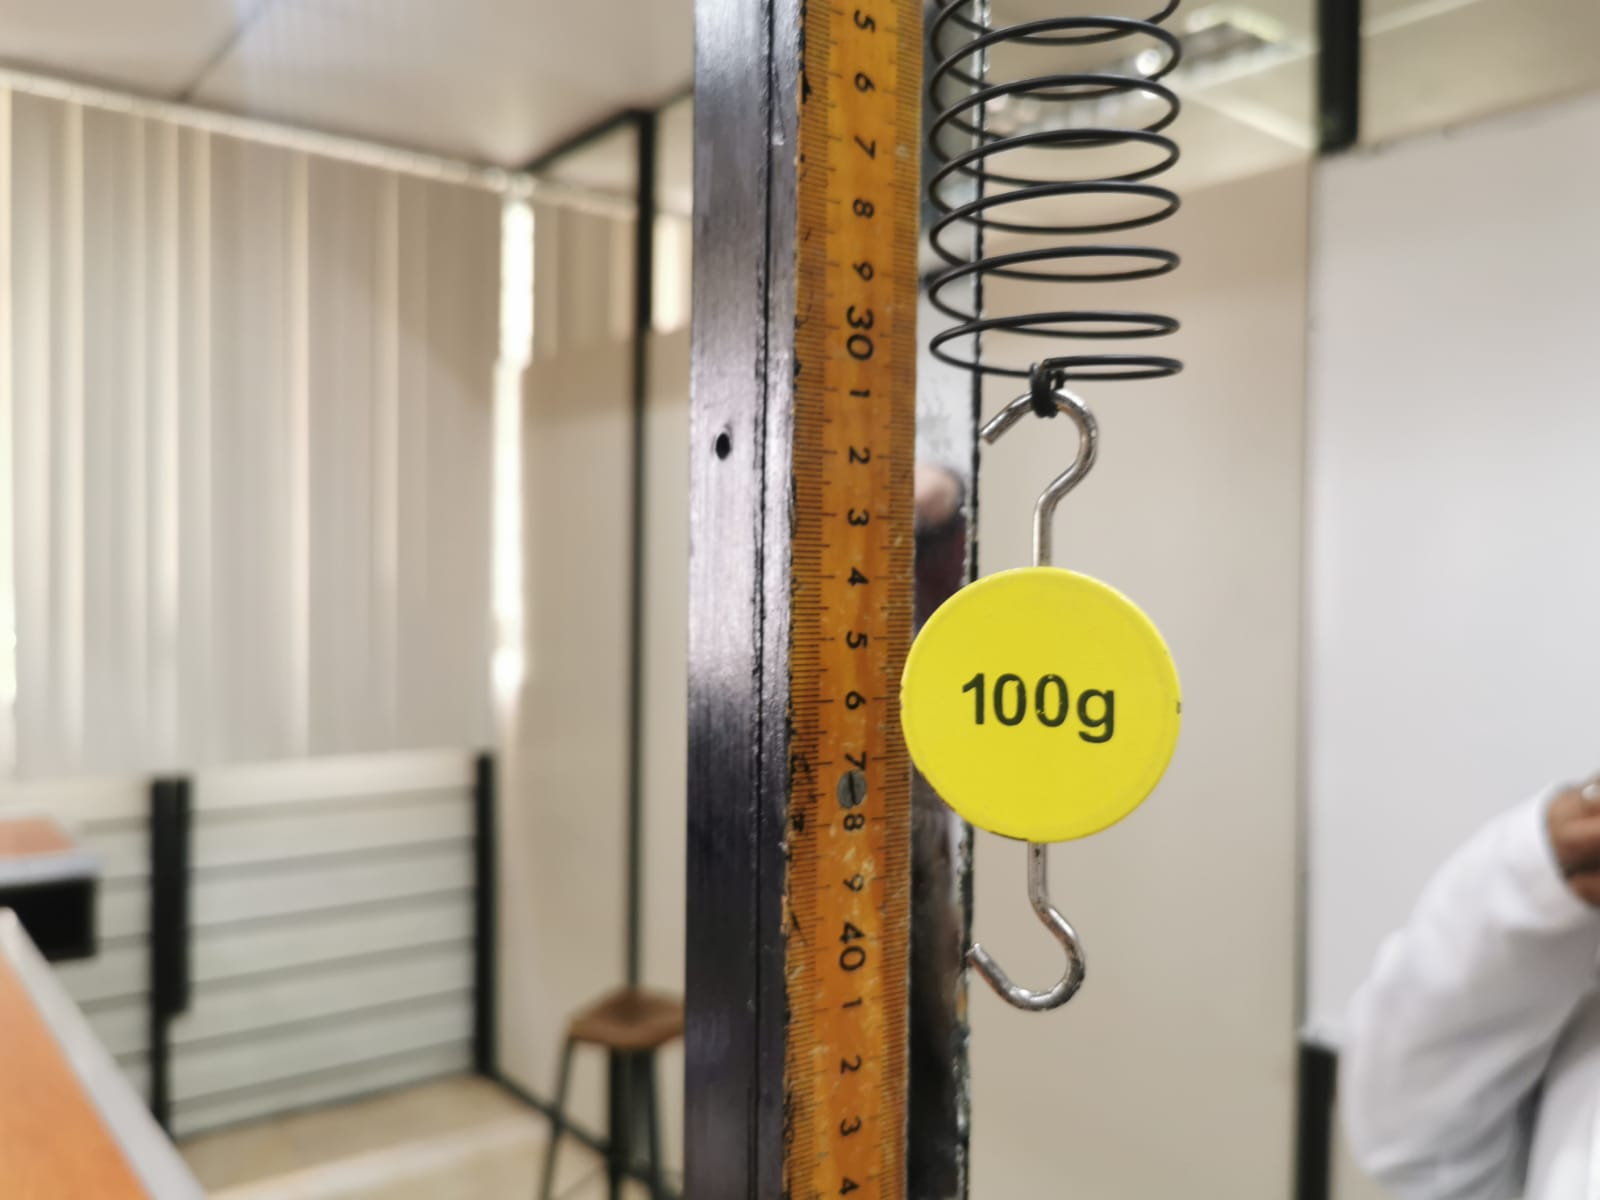
\includegraphics[width=3cm, height=4cm]{Imagenes/100gr.jpeg}
	\captionof{figure}{Masa de 100gr. Sostenida por el sistema de resorte lista para oscilarla.}
\end{center}
Y por ultimo calculamos la fuerza  total aplicada en el resorte.


\begin{center}
	\begin{adjustbox}{width=245pt}
		\begin{tabular}{|c|c|c|c|c|}
			\hline
			 &  &  &  & Método de mínimos cuadrados   \\
			\hline
			$m_{i}$ (Kg)&  $X_{i}$ (m)& $F_{i}$ (N)& $F_{i} x_{i}$ (Nm)& $x_1^2$ (m) \\
			\hline
			0.050& 0.017 & 0.166 &0.003	 &0.0003 \\
			\hline
			0.100& 0.038& 0.372 &0.014  & 0.0014 \\
			\hline
			0.150& 0.052 & 0.509& 0.026 & 0.0027 \\
			\hline
			0.200&0.072 &0.704 &0.051 & 0.0052\\ 
			\hline
			0.250&  0.090& 0.880& 0.079&0.0081 \\
			\hline
			0.300 &0.107 &1.046 & 0.112& 0.0114\\
			\hline
			0.350& 0.124 &1.213  &0.150 &0.0207 \\
			\hline
			0.400& 0.144 &1.408 &0.203 &0.0653\\
		   \hline
		   &  &  &$\sum(F_{i} X_{i} )=0.638 Nm $&$ \sum x_{1}^2=0.0653 m$\\
		  \hline
		\end{tabular}
	\end{adjustbox}
\end{center}


\begin{tikzpicture}
	\begin{axis}[
		title={Grafica 1},
		axis lines = left,
		xlabel = \(F_{i}[N]\),
		ylabel = {\(X_{i}[m]\)},
	]
	

	\addplot [
		domain=0:0.200, 
		samples=100, 
		color=black,
		]
		{9.75*x};

	\end{axis}
	\end{tikzpicture}


Determinamos que el tipo de relacion que existe entre las deformaciones y las fuerzas aplicadas son proporcionales, no cambian mucho.
Si se cumplió experimentalmente pues la función para describir entre deformación y fuerza es similar a la ecuación de la ley de Hooke.  

\subsubsection{Conclusión experimental}
En este experimento los resultados fueron los correctos para poder hacer la grafica y llegar a la conclusión si se cumplió la función de la ley de Hooke , con las mediciones y el estiramiento del resorte se cumplen la constante restitución de un resorte con su respectivo peso .

\section{Experimento 2. Relación entre la masa y el periodo.}
\subsection*{Procedimiento experimental:}
Pare este experimento probamos la relación entre la mesa y el periodo en un sistema masa resorte, por lo que usamos el sistema del primer experimento (el que solo cuenta con la base de barrillas y el resorte suspendido en estas).
La dinámica para realizar el experimento consistió en montar diferentes tipos de pesas, la mayor diferencia al experimento anterior es que gradualmente ponemos diferentes pesos al sistema de resorte y se deja dejo oscilar durante 20 oscilaciones valga la redundancia, medimos el tiempo y observamos el intervalo de tiempo para posteriormente registrar los resultados. En las siguientes imágenes se muestra el proceso de como se montaba cada fenómeno.

\begin{center}
	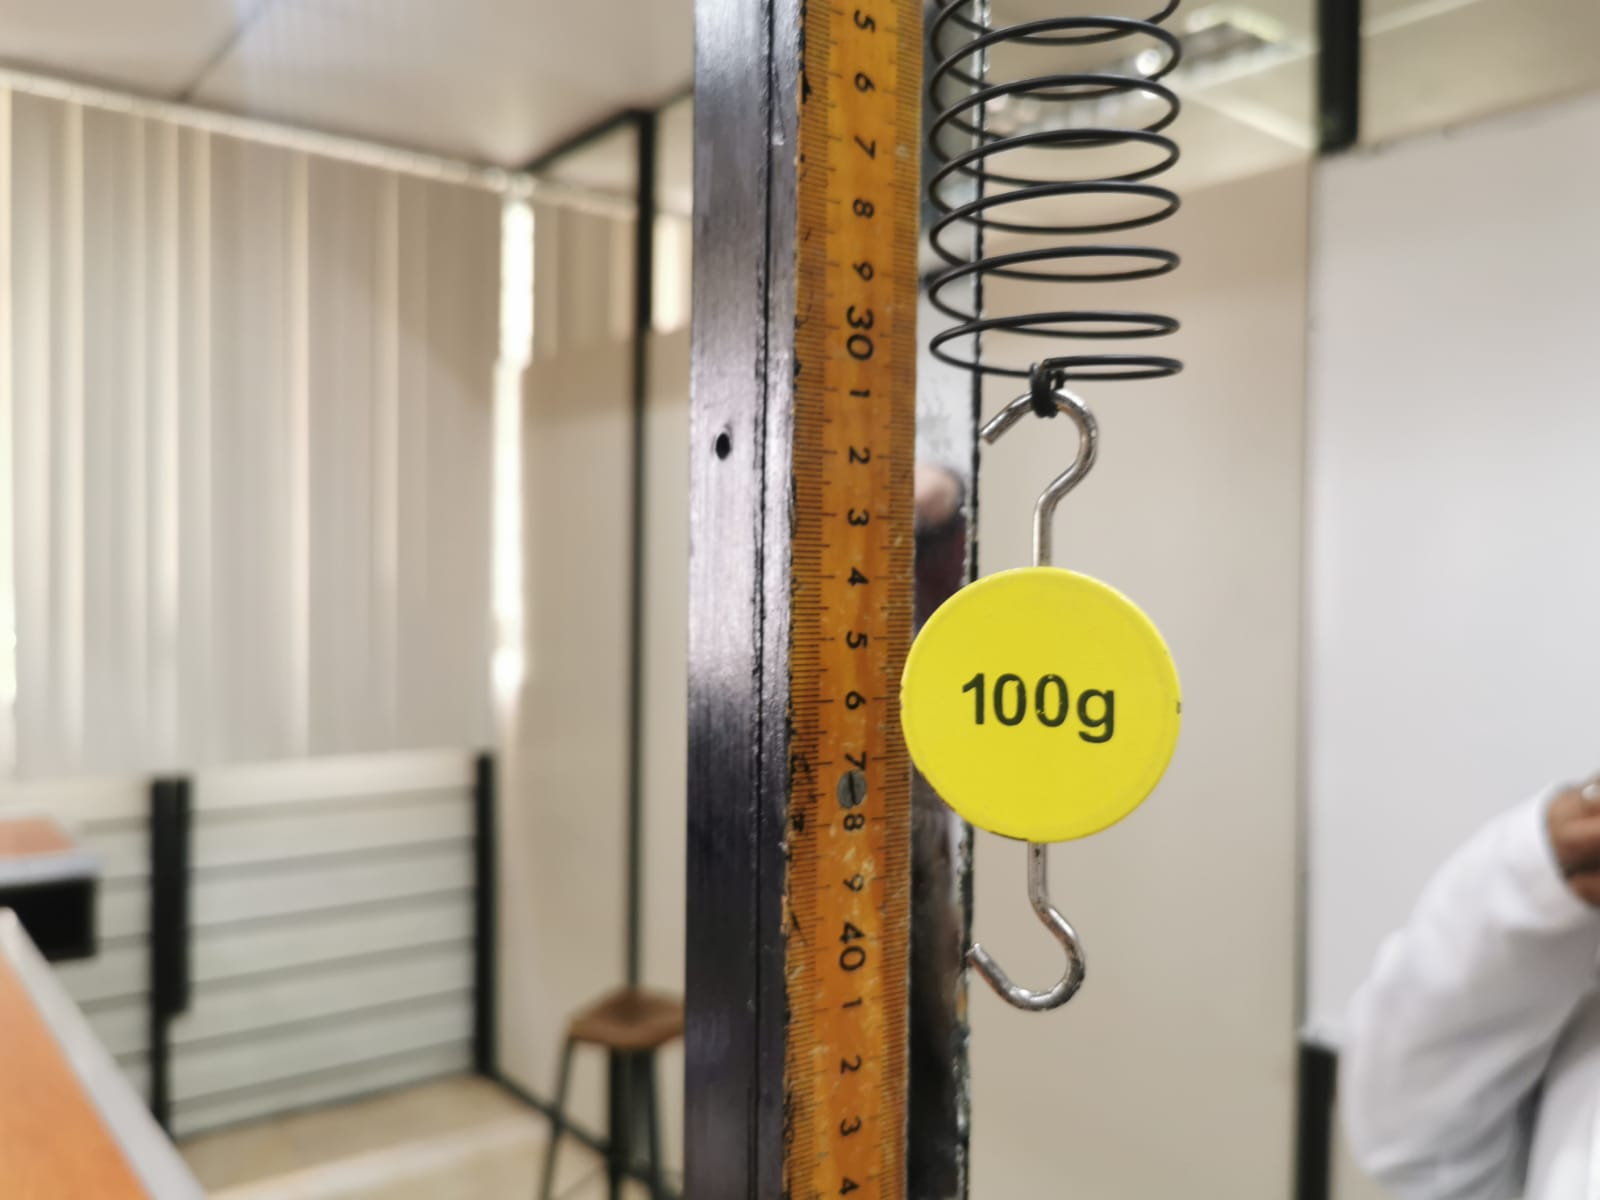
\includegraphics[width=3cm, height=4cm]{Imagenes/100gr.jpeg}
	\captionof{figure}{Masa de 100 gr. Sostenida por el sistema de resorte lista para oscilarla.}
\end{center}
\begin{center}
	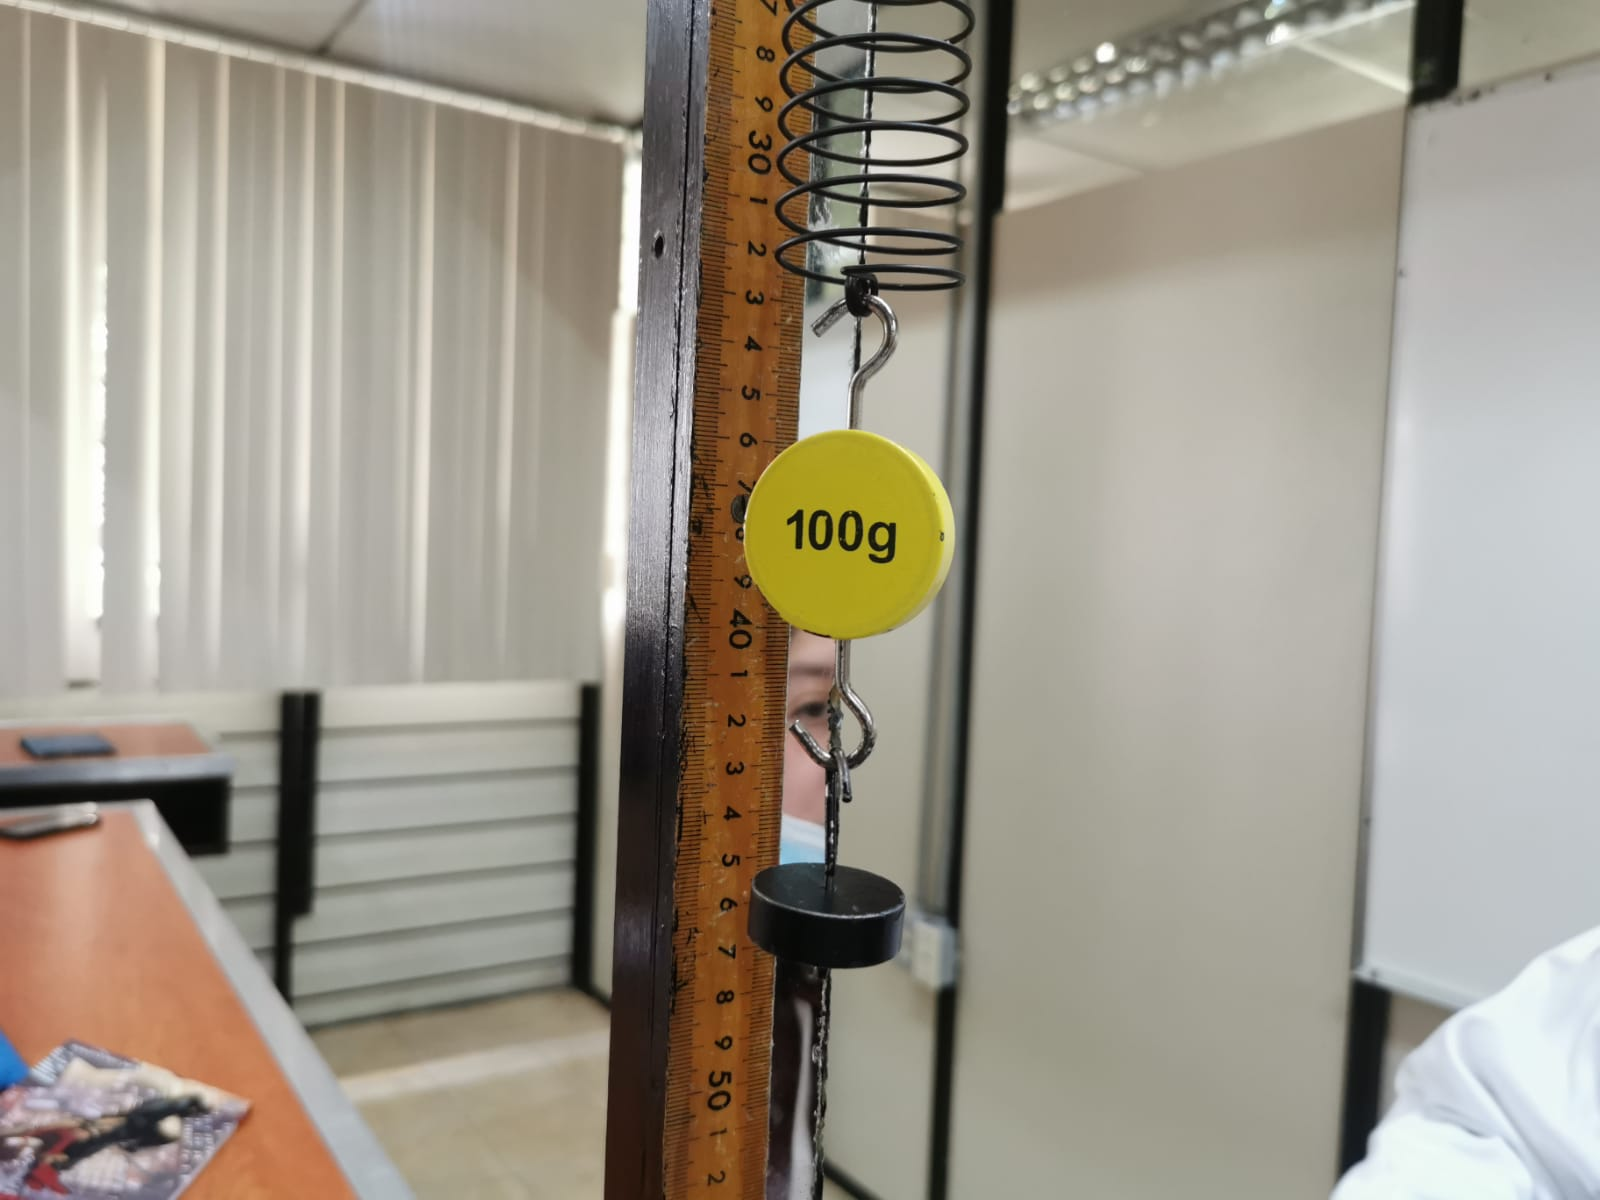
\includegraphics[width=3cm, height=4cm]{Imagenes/200gr.jpeg}
	\captionof{figure}{Masa de 200 gr. Sostenida por el sistema de resorte lista para oscilarla.}
\end{center}
\begin{center}
	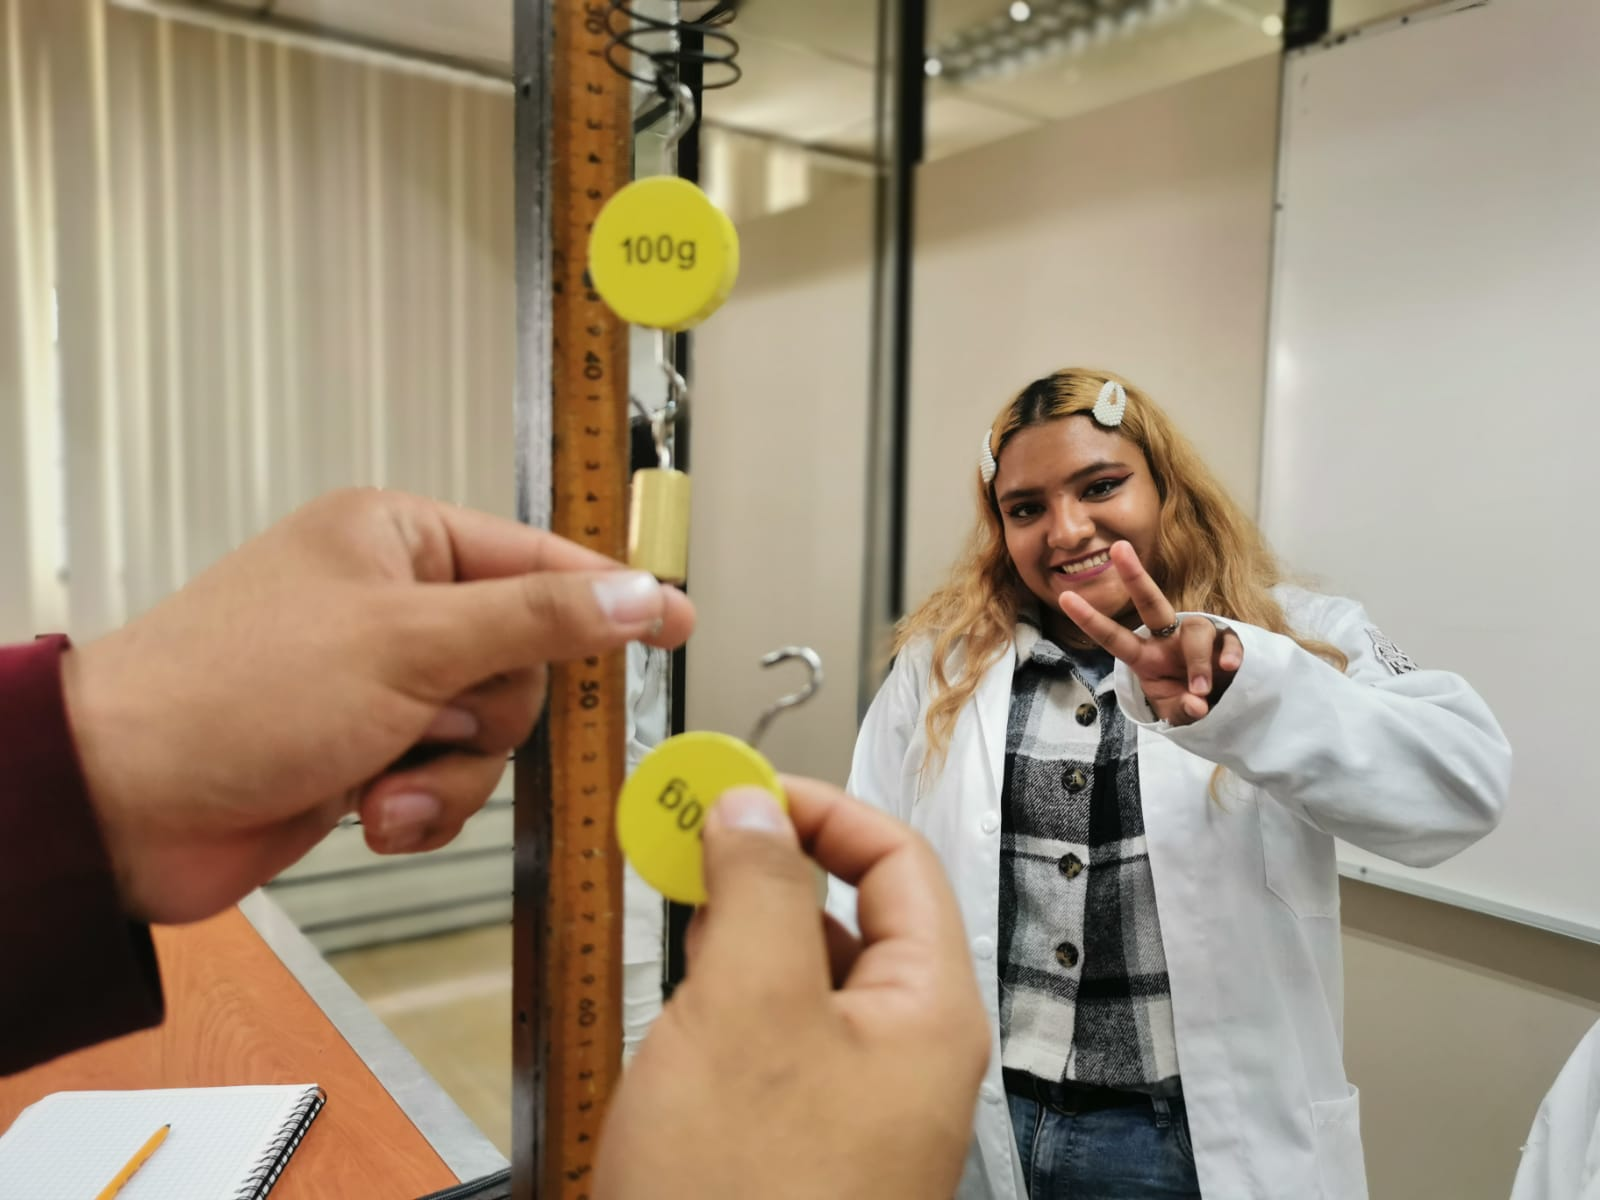
\includegraphics[width=3cm, height=4cm]{Imagenes/250gr.jpeg}
	\captionof{figure}{Masa de 250 gr. Sostenida por el sistema de resorte lista para oscilarla.}
\end{center}
\begin{center}
	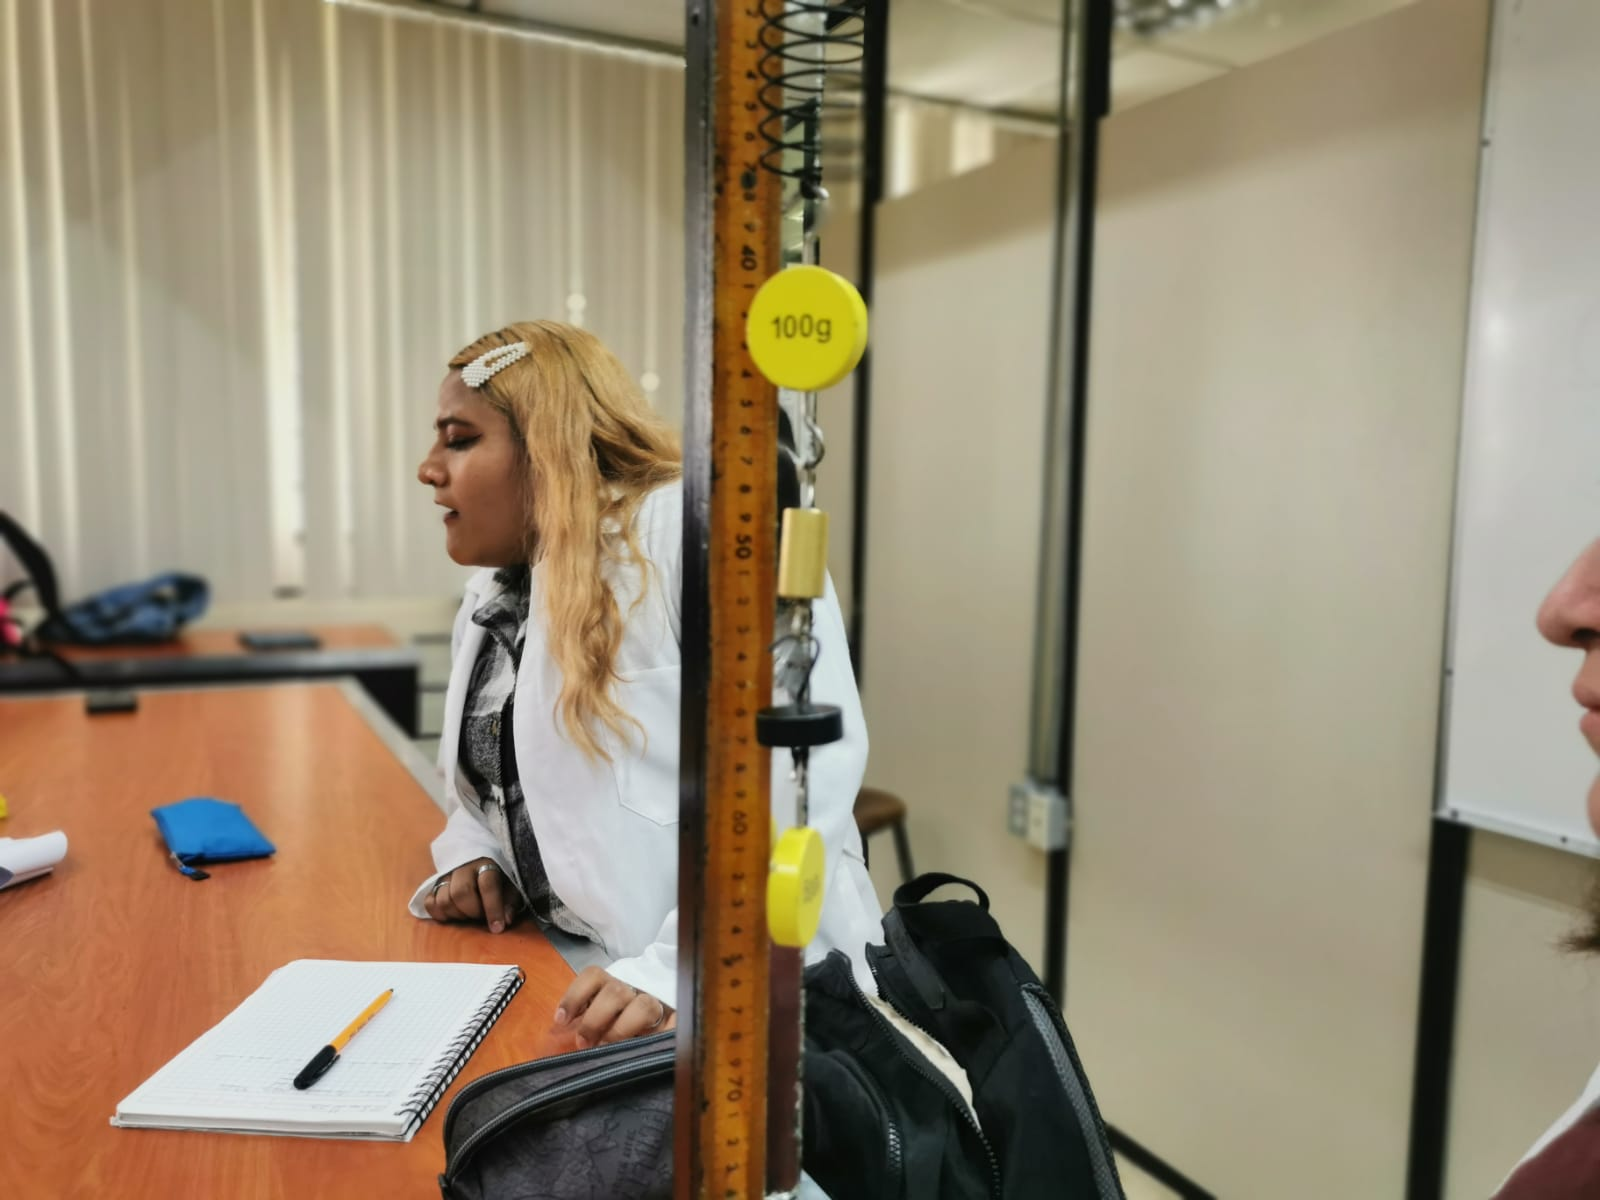
\includegraphics[width=3cm, height=4cm]{Imagenes/300gr.jpeg}
	\captionof{figure}{Masa de 300 gr. Sostenida por el sistema de resorte lista para oscilarla.}
\end{center}
\begin{center}
	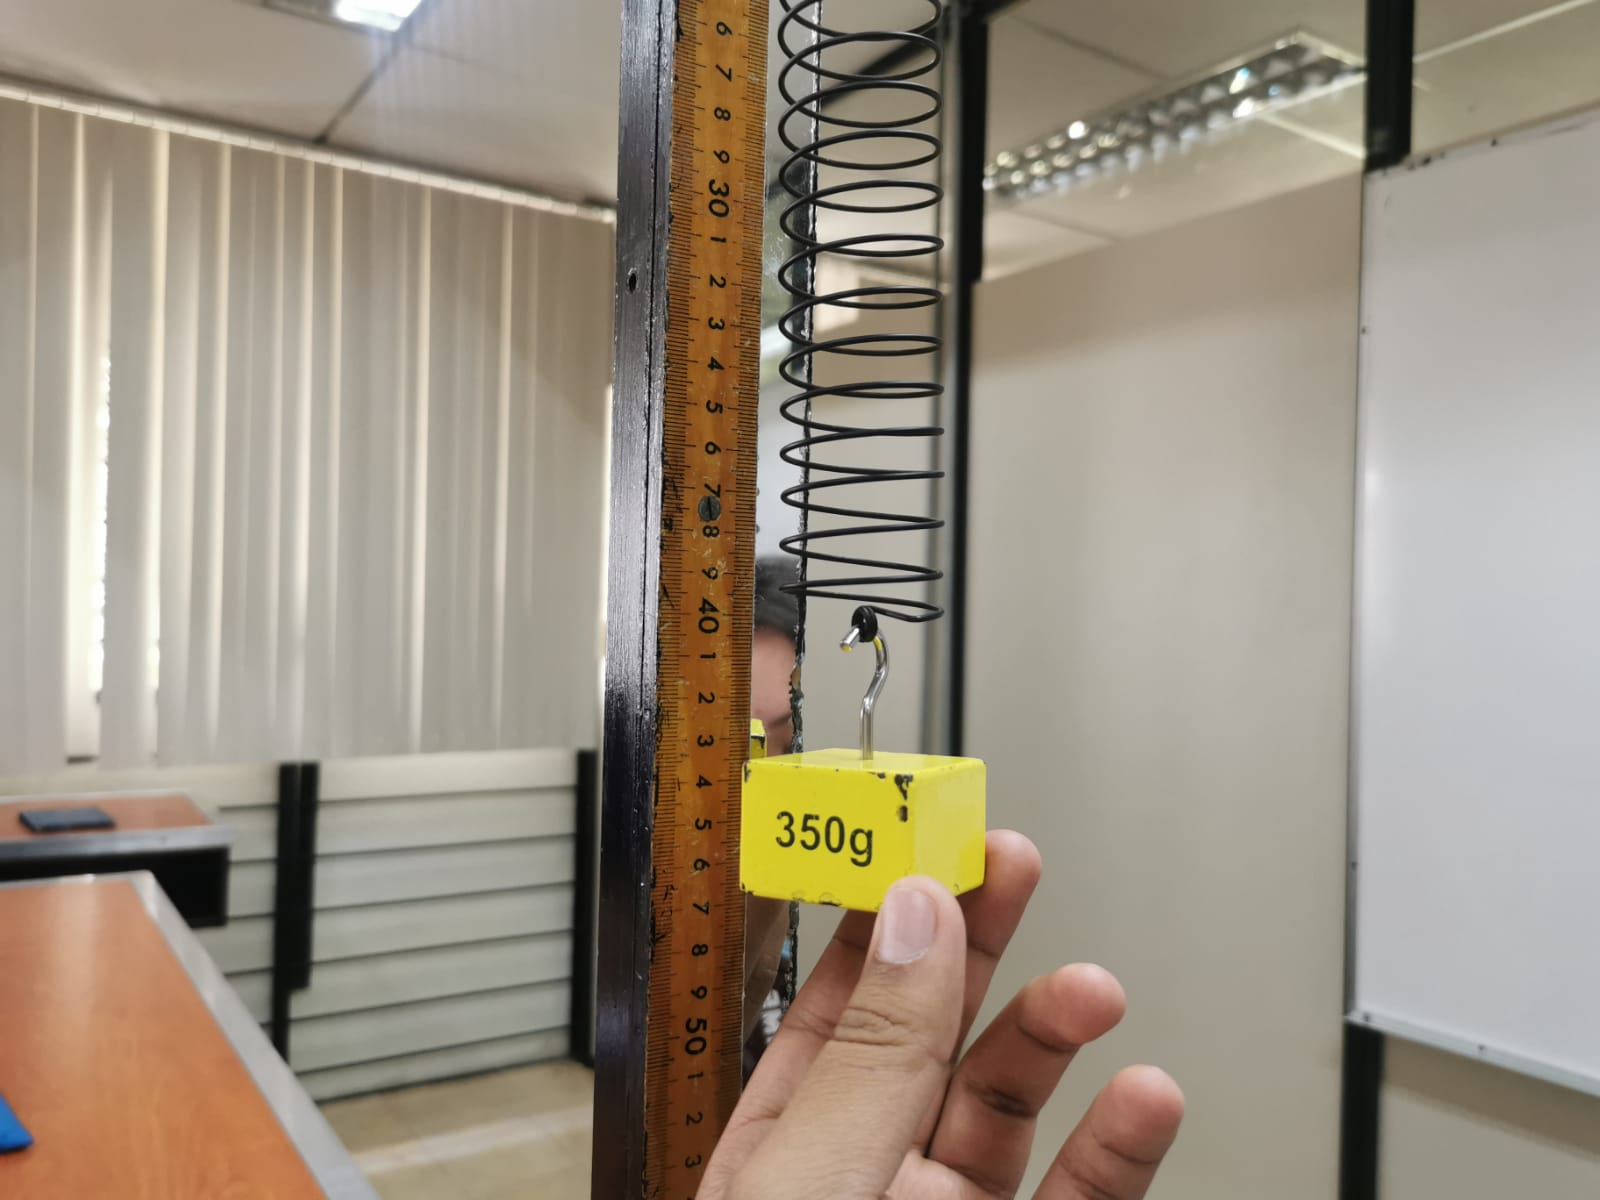
\includegraphics[width=3cm, height=4cm]{Imagenes/350gr.jpeg}
	\captionof{figure}{Masa de 350 gr. Sostenida por el sistema de resorte lista para oscilarla.}
\end{center}
Entre las observaciones mas destacables del procedimiento es que se dejaron 3 repeticiones antes de contar para que la masa-resorte oscilaran de manera más armónica.
\subsubsection{Desarrollo Experimental:}
El objetivo de todo este experimento es conseguir la ecuación de la interdependencia con respecto a “A”, despejando “K”
Partimos de \\ $\tau= 2\pi \sqrt{\frac{M}{k}}$\\
Elevando al cuadrado \\
$\tau^{2}=\frac{4\pi^{2}}{k}\dot M$\\
Definimos la constante de A como:\\
$A=\frac{4\pi^{2}}{k}$\\
Y al final tenemos: \\
$\tau^{2}=AM$\\
donde:\\
$\tau$=periodo de oscilación\\
M= masa efectiva\\
A=constante que depende del resorte\\
Después Determinamos el peso del resorte con el dinamómetro (Wr) y calculamos su masa, posteriormente calculamos $(m\prime)$\\
$m_{r}=\frac{W_{r}}{g}=\frac{0.55Kg\frac{m}{s^{2}}}{9.81\frac{m}{s^{2}}}=0.056Kg$\\
Posteriormente para saber el valor de la masa $m\prime$, calculamos el producto de mr por ($\frac{1}{3}$):\\
$m\prime=(\frac{1}{3})m_{r}=\frac{1}{3}\dot 0.056Kg=0.018Kg$\\
Lo anterior nos sirvió para poder completar los datos de M (masa efectiva) y de T*T (ESTO ES “T” AL CUADRADO, PERO ME DIO PEREZA BUSCAR COMO PONRLE LA POTENCIA POR ESO LO DEJE COMO PRODUCTO), \\ Por medio de la siguiente tabla:


\begin{center}
	\begin{adjustbox}{width=245pt}
		\begin{tabular}{|c|c|c|c|c|c|}
			\hline
			$m_{i}$[Kg] & $M_{i}[Kg]$ & $t_{i}$[s] & $T_{i}$[s]  &$T^{2}_{i}[s^{2}]$  \\
			\hline
			0.100 & 0.10019 & 6.0000& 0.3000 & 0.0900 \\
			\hline
			0.200 & 0.20019 & 8.9000& 0.4450 & 0.1980 \\
			\hline
			0.250 & 0.25019 & 10.3000 & 0.5150 & 0.2652 \\
			\hline
			0.300 & 0.30019 & 11.2000 & 0.5600 & 0.3136 \\
			\hline
			0.350 & 0.35019 & 12.3000 & 0.6150 &0.3762 \\ 
			\hline
			0.400 & 0.40019 & 13.3000 & 0.6650 & 0.4422\\
			\hline
			0.450 & 0.45019 & 14.1900 & 0.7095 & 0.5034\\
			\hline
		\end{tabular}
	\end{adjustbox}
\end{center}
\begin{tikzpicture}
	\begin{axis}[
		title={Grafica 2},
		axis lines = left,
		xlabel = \(M_{i}(Kg)\),
		ylabel = {\(T_{i}(s)\)},
	]
	

	\addplot [
		domain=0:0.60000, 
		samples=100, 
		color=black,
		]
		{1.1846*x - 0.0342};
	
	\end{axis}
	\end{tikzpicture}
Metimos los datos a una graficadora donde consideramos que “x” como “Ti*Ti[s al cuadrado]” y “y” como “Mi[Kg]”
%-----------------------"Grafica"-------------------------%
\begin{center}
	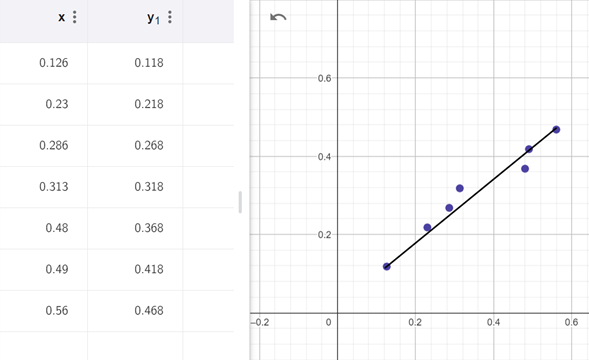
\includegraphics[width=10cm, height=7cm]{Imagenes/graficarogue.png}
	\captionof{figure}{Grafica del peso inicial con respecto al tiempo al cuadraro}
\end{center}
Valor de la pendiente trazada: 0.8432 u \\
(Este valor se obtuvo después de determinar las coordenadas del primer y último punto dado por la gráfica, no es automático de la graficadora, pero se hizo en base de un software de matemáticas).
Y para finalizar con esta parte del desarrollo ajustamos la recta por el método de mínimos cuadrados, para obtener el valor de la constante A de la pendiente.
En primer lugar calculamos las sumas de $(T_{i}^{2}),M_{i},(T_{i}^{2})^{2},(T_{i}^{2})\dot M_{i}$\\
$\sum(T_{i}^{2})=0.126+0.23+0.286+0.313+0.48+0.49+0.56=2.485$\\
$\sum M_{i}=0.118 + 0.218 + 0.268 + 0.318 + 0.368 + 0.418 + 0.468=2.247$\\
$\sum(T_{i}^{2})^{2}=0.126^2 + 0.23^2 + 0.286^2 + 0.313^2 + 0.48^2 + 0.49^2 + 0.56^2=1.032$\\
$\sum(T_{i}^{2})^{2}\dot M_{i}=(0.126*0.118)+(0.23*0.218)+(0.286*0.268)+(0.313*0.318)+(0.48*0.368)+(0.49*0.418)+(0.56*0.468)=0.884$\\
Después calculamos la pendiente (m) y la ordenada la origen (b), teniendo en cuenta que n=7:\\
$m=\frac{n*\sum(T_{i}^{2}) * M_{i}-\sum(T_{i}^{2})*\sum M_{i}}{n*\sum(T_{i}^{2})^{2}-(\sum(T_{i}^{2}))^{2}}=\frac{(7)(0.884)-(2.485)(2.247)}{(7)(1.032)-(2.485)^2}=0.127$\\

$b=\frac{\sum M_{i}-m*\sum T_{i}^{2}}{n}=\frac{2.247-(0.127)(2.485)}{7}=0.275$\\

Y al final la ecuación nos quedó de la siguiente manera:\\
$y=mx+b  \rightarrow  y=0.127x+0.275$\\
$\therefore M=AT^2    \rightarrow     T^2=AM$\\
\subsubsection{Discusión:}
La relación entre el cuadrado del periodo y la masa del oscilador armónico esta dada por una constante, la cual define la rigidez del resorte y la frecuencia angular del oscilador, la constante k, está contenida dentro de A, pero, en otras palabras, si mantienes constante la constante del resorte (k), un incremento en la masa del oscilador resultará en un período mayor y, por lo tanto, un movimiento más lento del oscilador.
Cálculo de “k” por este experimento:
Empezamos por la ecuación (2) de la practica donde:\\
$-kx=Ma     \rightarrow     -k=Ma/x       \rightarrow  (-)(-k=Ma/x)    \rightarrow     k=-Ma/x$\\
$\therefore k_{D} = 0.806 \frac{N}{m}$\\
Comparación de resultados y cálculos de la precisión:\\
Comparando el valor de kd y el valor de la pendiente que obtuvimos gráficamente que la tomaremos como k:\\
$Presicion = \frac{\bigtriangleup K}{K}100(\%)$\\
$\bigtriangleup k=k-kd=0.127-0.806=0.679$\\
$\frac{k+kd}{2}=\frac{0.127+0.806}{2}=0.466$\\\
La precision es del 46$\%$

En resumen, este experimento nos proporcionó una comprensión más profunda del comportamiento de un oscilador armónico simple y cómo factores como la masa y la constante del resorte afectan sus propiedades fundamentales. Estos conceptos son cruciales en la física y tienen aplicaciones en numerosos campos, desde la mecánica hasta la ingeniería y la astronomía. El estudio de los osciladores armónicos sigue siendo relevante y ofrece valiosas lecciones sobre los principios fundamentales del movimiento periódico en la naturaleza.

\section{Experimento 3.  Obtención de la aceleración de la gravedad de la localidad $(g)$}
Para este experimento manipularemos un objeto con propiedades físicas oscilatorias armónicas simples, donde podremos analizar su efecto estirando el resorte helicoidal midiéndolo con la balanza Jolly que lo afectará una masa m (100g), también calcularemos el periodo teniendo en cuenta sus incertidumbres en los datos tabulados. 
Para la realización de nuestro experimento, utilizamos una masa m para colocarla en la parte inferior del resorte helicoidal, contando el periodo que se realiza después de las 20 oscilaciones completas.
\begin{center}
	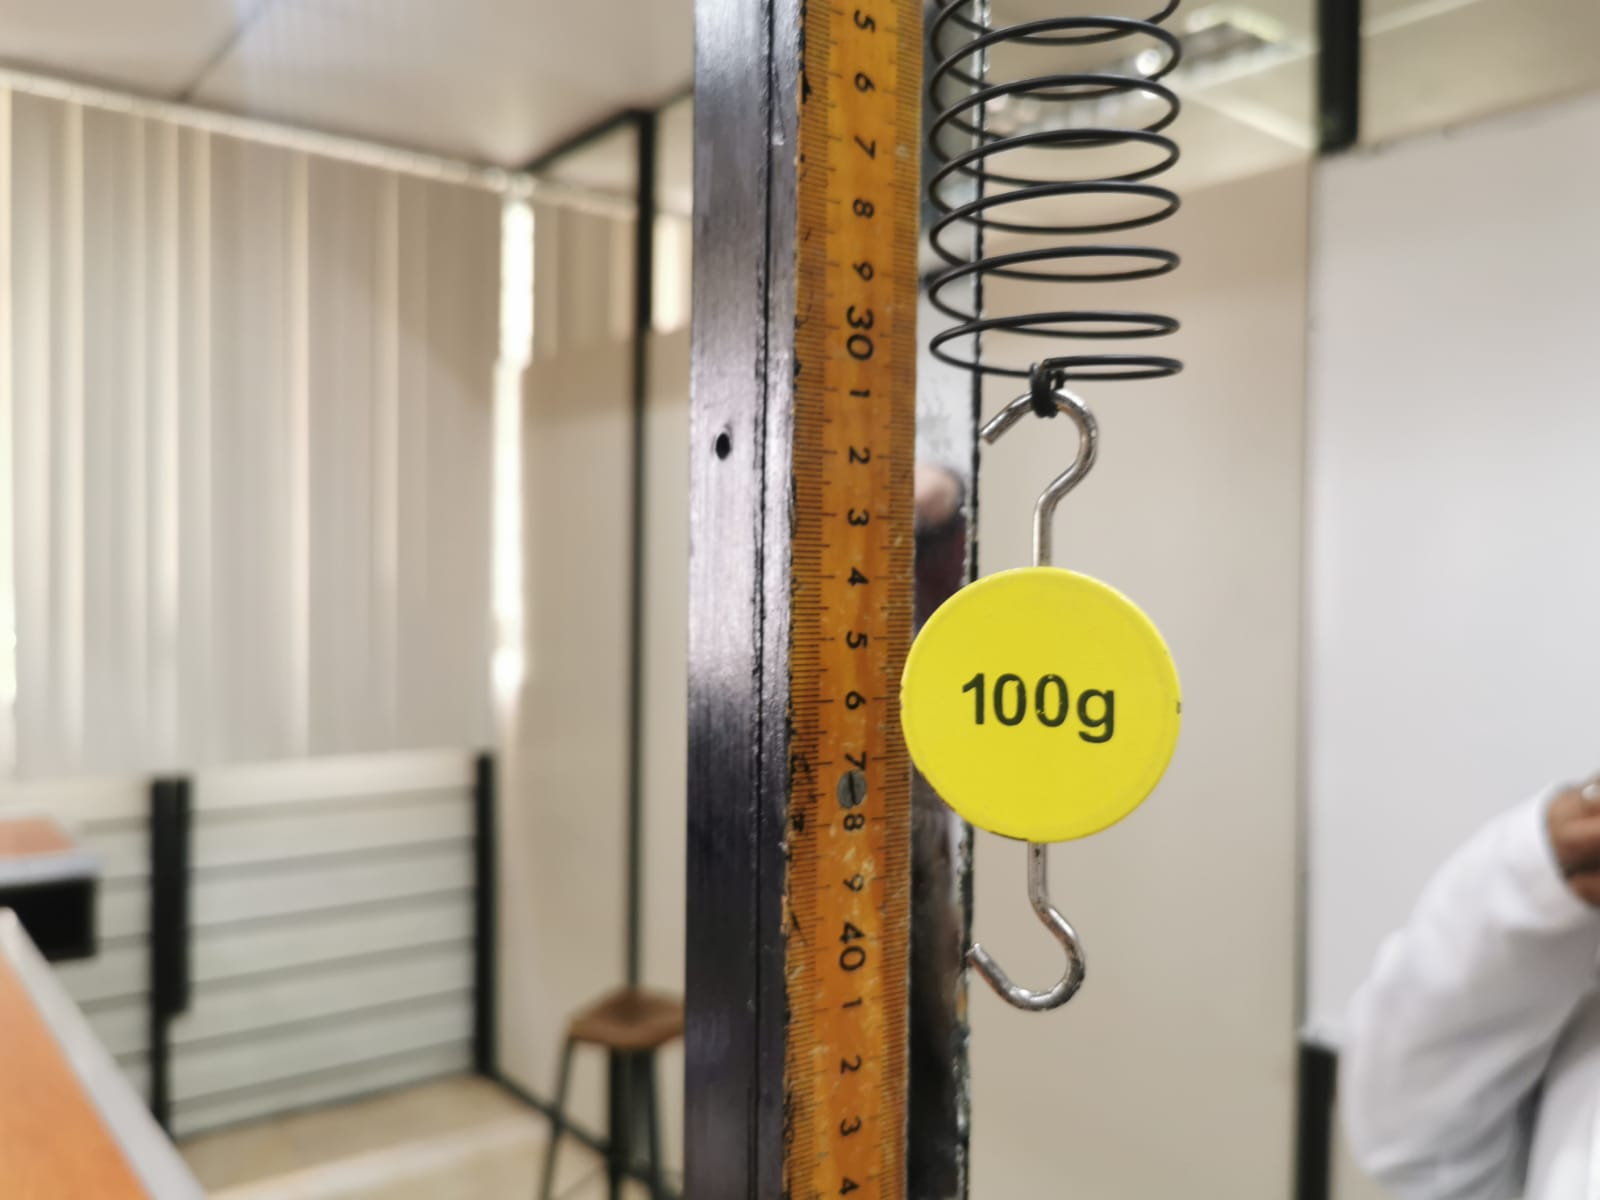
\includegraphics[width=3cm, height=5cm]{Imagenes/100gr.jpeg}
	\captionof{figure}{La balanza Jolly con el resorte helicoidal con una masa de 100gr.}
\end{center}
Para obtener un resultado más preciso y rápido, 3 de mis compañeros tomaron el tiempo para que los resultados del tiempo (s) se promediaran tabulando finalmente nuestros resultados. 
Cálculo del periodo tomando en cuenta que la gravedad de la ciudad de México es de 9.78$\frac{m}{s^{2}}$\\
$\tau = 2\pi \sqrt{\frac{x}{g}}$\\
$\tau = 2\pi \sqrt{\frac{0.31 m}{9.78 m/s^2 }}$\\

$\tau =1.118s$\\
Calculando la incertidumbre del periodo con los datos tabulados. \\
$
\delta T = 2\pi \sqrt{\frac{\delta x}{g}}\\
\delta T = 2\pi \sqrt{\frac{0.32}{9.78 m/s^2}}\\
\delta T = 1.136s\\ $

Tabla de tabulación 


\begin{center}
	\begin{adjustbox}{width=245pt}
		\begin{tabular}{|c|c|c|c|c|c|}
			\hline
			m[kg] & x[m] & $\delta$x[m] & t[s]  &T[s] &$\delta$T[s]\\
			\hline
			0.1  & 0.31 & 0.32 & 8.39 &1.118  &1.136  \\
			\hline
	
		\end{tabular}
	\end{adjustbox}
\end{center}

Iniciamos partiendo de la Ley de Hooke donde \\
 F= -k*x \\
 F= ma \\
Sustituyendo valores \\

 F=0.1 kg*9.78 $m/s^2$   \\
 F= 0.978 N \\
Entonces: \\
 F= -k*x \\
0.978 N= -k * 0.31m \\
Despejando nuestra constante de proporcionalidad sobre nuestro resorte. \\
 k=0.31 m-0.978 $ kg*m/s^{2}$\\
 k= -0.668 $kg*m/s^{2} $\\
Calculamos nuestra masa M, donde M = $m + \frac{1}{3} m_{r}$ \\
 $(m_{r}$, Masa del resorte)\\
Sustituyendo datos tabulados con la ecuación obtenemos \\
 $M=0.1+ \frac{1}{3}  (0.00056)$\\
$M=0.1018 kg$\\

Sustituyendo la ecuación (4) del experimento 1, se sustituye con los datos tabulados y constantes calculadas del experimento 3, tenemos que:\\

$
-k=M\frac{d^{2}x}{dt^{2}}
$\\
Pero sabemos que la ecuación\\
$ \frac{d^{2}x}{dt^{2}}=a$\\
Sustituyendo con las variables ya obtenidas con la constante de la aceleración (gravedad) ya otorgada sabiendo que tiene un valor de $9.78 m/s^2$  tenemos que: \\

-k=Ma
$\frac{-k}{M}=a$\\
$a=\frac{(-(-0.668 (kg*m)/s^2 ) )}{(0.1018 kg)}$\\
$a=(0.668  (kg*m)/s^2 )/(0.1018 kg)$\\
$a=6.56 m/s^2 $ \\
La incertidumbre la calculamos con \\
$\frac{\delta g} {g}= \frac{\delta x }{x}+2\frac{ \delta T} {T}$\\
Despejando la incertidumbre de la gravedad \\
$\delta g =g( \frac{\delta x} {x}+2 \frac{\delta T} {T})$\\
Sustituyendo los datos obtenemos: \\
$\delta g =g(\frac{ \delta x}{x}+2 \frac{\delta T}{T})$\\
$\delta$g =$6m/s^2 (\frac{0.32m}{0.31m}+\frac{2 1.136s}{1.118s}$\\
$\delta$g =$8.8 m/s^2 $\\
Entonces. \\
El valor de la aceleración de la gravedad (g) en donde se llevó a cabo el experimento 1. \\
$g_{0} =g \pm \delta g=6.56 \pm 8.8 m/s^2 $\\


%-----------------------Concluciones-------------------------%
\section{Conclusiones.}

\subsection*{Hernández Huerta Jose Emilio.}
Con base en lo experimentado con la aplicacion de un sistema masa resorte podemos calcular la aceleracion de la gravedad mediante calculos que involucran la posicion y su periodo, el cual tiene una peculiar coincidencia con la relacion entre sus masa y su periodo, pues son formas diferentes de allar el periodo entre con respecto a variables diferentes lo que me hace concluir que para despreciar la masa realmente trabajariamos con su peso $m*g$.
\subsection*{Hernández Sanluis Danna Estefany.}
En esta práctica se pusieron a prueba varios conceptos vistos en clase y ver la demostración de como es el estiramiento del mismo resorte con ayuda de la masa , y al momento de graficar los datos vimos que no tienes una gran diferencia en tiempo y distancia , vas de la mano ambos valores , también una ley importante que vimos fue la ley de Hooke que nos permitió saber si se cumplía la función de la misma con los valores obtenidos , todo este procedimiento nos servirá en temas mas adelante para poder calcular el movimiento general de las ondas mecánicas . 
\subsection*{Nataly Bejarano Garduño.}
En esta practica, se observa el Fenomeno del Movimiento Armonico Simple comprobando como tomar un periodo de onda y hacer una relción mediante graficas para observar esta relación de masa resorte, y apreciar la Ley Houk sobre Señor Doctor Slinky. 
\subsection*{Mojica Reyes Rogelio.}
Este experimento tomo como principal objetivo la relación que existe entre la masa y el periodo en un sistema de movimiento armónico simple, por lo que nuestro objetivo particular era el demostrar si existía algún cambio al sistema montado (varillas y resorte) con respecto al agregar ciertos tipos de masas y al referirnos a ciertos tipos nos referimos a ciertas magnitudes de peso.

Notamos que si existía un tipo de cambio, pero era con respecto al tiempo que está relacionado con la aceleración, ya que al existir más peso el tiempo de oscilación se prolonga más y tiende a variar, por lo que podemos decir que existe una gran relación entre la masa y el periodo.
\subsection*{Morlan Juárez Bruno Tonatiuh.}
Durante este experimento observamos el fenómeno del Movimiento Armónico simple, aplicando fuerzas de diferente magnitud notando y comprobando su comportamiento con las fórmulas ya establecidas durante el experimento, los datos obtenidos han sido recolectados según lo aprendido en clases, solucionando algunas dudas durante el experimento se hizo aún más claro el tema, pero, el estudio y la dedicación harán que el curso vaya al mismo resultado. 
\subsection*{Santos Marañón María Renée.}
Un sistema tiene diferentes factores como el peso o la gravedad, también tendrá un número de oscilaciones diferentes, mientras menos peso puede haber más oscilaciones en un cierto número de tiempo, en esta práctica pudimos comprobar lo antes dicho, los cambios que tiene un péndulo cuando le agregas un peso e incluso una herramienta más como el dinamómetro pues este último ayuda a saber la fuerza con la cual el peso estira el resorte.

Se vio como un resorte se comporta como un oscilador, la manera en que la fuerza de restricción permitía al mismo volver al estado de equilibrio.

%-----------------------Bibliografia-------------------------%

\begin{thebibliography}{0}
	\bibitem{citekey}[(Movimiento ARM nico simple y oscilador amortiguado, s.f.)]
	\bibitem{citekey}[MANUAL DE PRACTICAS DE LABORATORIO DE ONDAS MECANICAS. (s.f.). IPN.]
	\bibitem{citekey}[Fernández, J. L. (s.f.). Movimiento armónico simple (M.A.S.). Fisicalab. https://www.fisicalab.com/apartado/concepto-oscilador-armonico]
	\bibitem{citekey}[(Simple Harmonic motion. (s.f.). http://hyperphysics.phy-astr.gsu.edu/hbasees/shm.html)]
\end{thebibliography}

\end{multicols}

\end{document}
